\section{算子的定义}
\label{sec:lop-definition}

在$L^2(0,1)$中把函数投影到常数子空间，得到它的平均值组成的常函数。对连续函数$f$作积分$x\mapsto\int_0^xf(t)\,\mathrm dt$，得到一个可导函数。对可导函数求导，又回到一个可能不再可导的函数。

三种操作的共同点是：输入一个函数，输出另一个函数，并且保持线性组合。差别在于它们对输入的要求：投影和积分对空间中每个元素都有意义，求导只对一部分函数有意义。矩阵不会遇到这种差别，算子却必须从这里说起。

\subsection{线性算子}
\label{sec:lop-linear-operators}

矩阵$\bm A\in\mathbb R^{m\times n}$作用于每个$\bm x\in\mathbb R^n$，输入、输出的所在空间由矩阵形状直接给出。函数空间中，作用规则往往先以公式出现，例如“求导”或“对核积分”，而公式本身并不说明对哪些函数有意义。因此定义算子时，要把允许的输入集合与输出所在的空间作为算子的一部分写出来。

\begin{definition}[线性算子]
\label{def:lop-linear-operator}
设$X,Y$是同一标量域$\mathbb F$（$\mathbb R$或$\mathbb C$）上的线性空间，$D(T)\subseteq X$是线性子空间。映射$T:D(T)\to Y$若满足
\begin{equation}
 T(\alpha x+\beta z)=\alpha Tx+\beta Tz\qquad(x,z\in D(T),\ \alpha,\beta\in\mathbb F),
 \label{eq:lop-linearity}
\end{equation}
则称$T$为从$X$到$Y$的\term{线性算子}（linear operator）。$D(T)$称为$T$的\term{定义域}（domain），$Y$称为它的取值空间。集合
\begin{equation}
 \operatorname{Ran}T=\{Tx:x\in D(T)\},\qquad\ker T=\{x\in D(T):Tx=0\}
 \label{eq:lop-range-null}
\end{equation}
分别称为$T$的\term{像空间}（image space）和\term{零空间}（null space），也简称像与核。
\end{definition}

定义要求$D(T)$是线性子空间，这样$\alpha x+\beta z$仍是允许的输入，线性条件才有意义。由线性得$T0=0$。像与零空间都是线性子空间：两个输出的线性组合是相应输入线性组合的输出，两个被送到零的输入之和也被送到零。

矩阵的列空间与零空间在这里仍然对应。取值空间$Y$是事先指定的，像$\operatorname{Ran}T$则由算子实际产生，二者相等时才称$T$为满射。

零空间描述哪些输入的差别在输出中完全看不见：
\[
 Tx=Tz\quad\Longleftrightarrow\quad x-z\in\ker T.
\]
所以$T$是单射当且仅当$\ker T=\{0\}$。这与矩阵情形相同，只是这里的“输入”可能是函数的等价类，零空间也要在相应意义下理解。

有限维中的秩—零化度公式却没有对应物。方阵是单射当且仅当是满射；无限维中二者彼此独立，第~\ref{sec:lop-adjoint}节的右移算子是单射但不是满射。

$D(T)=X$时，称$T$定义在整个$X$上，简记$T:X\to Y$；本章若不特别写出定义域，算子都是这种情形。另一种情形是$D(T)$只是$X$的真子空间，求导就是典型。把它看成从$C[0,1]$到$C[0,1]$的算子时，只有可导函数才是允许的输入。

两种情形必须分开：后面讨论有界性时，定义域上的范数与取值空间上的范数各自指定，而定义在真子空间上的算子是否有界，取决于在这个子空间上用什么范数衡量输入。

取值空间为标量域$\mathbb F$时，线性算子就是第~\ref{chap:linear-functionals}章的线性泛函，相当于只有一行的矩阵。下面关于算子的结论都包含泛函的情形，泛函那里建立的表示和延拓工具也会在伴随与基本定理中再次用到。

\subsection{常见算子}
\label{sec:lop-common-operators}

下面几个例子在本章反复出现。对每个例子，我们写出输入空间、输出空间与作用规则，再核对线性，并说明它相当于什么样的矩阵。重点是看出“公式能写出来”与“算子已经定义好”之间还差哪些检查。

\paragraph{恒等映射与正交投影}
对任意线性空间$X$，\term{恒等算子}（identity operator）$I_Xx=x$定义在整个$X$上。线性由定义直接得到：两边都等于$\alpha x+\beta z$。它相当于单位矩阵，不同空间各有自己的恒等算子，复合时要分清$I_X$与$I_Y$。

设$H$是Hilbert空间，$M\subseteq H$是闭子空间。第~\ref{chap:function-inner-product-spaces}章说明每个$x\in H$在$M$中有唯一的最近点$P_Mx$，并且$x-P_Mx\perp M$。由此得到正交投影$P_M:H\to H$。

正交投影的线性需要验证。向量$\alpha P_Mx+\beta P_Mz$属于$M$，并且残差
\[
 \alpha x+\beta z-(\alpha P_Mx+\beta P_Mz)=\alpha(x-P_Mx)+\beta(z-P_Mz)
\]
与$M$正交。满足这两条的元素唯一，所以它就是$P_M(\alpha x+\beta z)$。

例如在$L^2(0,1)$中取$M$为常函数子空间，单位向量$1$张成$M$，于是
\[
 P_Mf=\langle1,f\rangle\cdot1=\Bigl(\int_0^1f\,\mathrm dt\Bigr)\cdot1.
\]
这个算子的“矩阵”处处等于$1$：它的核是$k(x,y)\equiv1$，每一行都把输入平均一次。

\paragraph{固定函数相乘}
设$(\Omega,\mathcal F,\mu)$是测度空间，$\varphi\in L^\infty(\mu)$，$1\leq p\leq\infty$。对$f\in L^p(\mu)$令$M_\varphi f=\varphi f$，称为\term{乘法算子}（multiplication operator）。按分量看，它把第$x$个分量乘以$\varphi(x)$，正是对角矩阵的连续版本。

下面逐项核对。若$f=g$几乎处处，则$\varphi f=\varphi g$几乎处处，所以作用对等价类有确定的意义。由几乎处处成立的不等式
\[
 \lvert\varphi f\rvert\leq\lVert\varphi\rVert_\infty\lvert f\rvert,
\]
输出仍在$L^p(\mu)$中。线性来自乘法对加法的分配律。

对角元素无界时情况就变了。在$(0,1)$上取$\varphi(x)=x^{-1}$，函数$f=1$属于$L^2(0,1)$，而$\varphi f=x^{-1}$不平方可积。公式仍可写出，却不再给出$L^2$到$L^2$的算子。

\paragraph{积分变换}
设$(X,\mu)$与$(Y,\nu)$是测度空间，$k:X\times Y\to\mathbb F$可测。形式上令
\begin{equation}
 (Tf)(x)=\int_Yk(x,y)f(y)\,\mathrm d\nu(y),\qquad x\in X,
 \label{eq:lop-integral-operator}
\end{equation}
称$k$为\term{积分核}（integral kernel），$T$为以$k$为核的\term{积分算子}（integral operator）。按式~\eqref{eq:lop-matrix-integral}的类比，第一个变量$x$是输出的位置，也就是行；第二个变量$y$是输入的位置，也就是列。固定$x$，$k(x,\cdot)$就是这一行的全部元素。

只要右端对每个输入有意义，线性就由积分的线性得到。问题在于“有意义”需要核、参考测度和输入函数共同决定。在$[0,1]$上取Lebesgue测度与核$k\equiv1$，则
\[
 (Tf)(x)=\int_0^1f(y)\,\mathrm dy.
\]
对$f(y)=y^{-1/2}$积分为$2$，对$f(y)=y^{-1}$积分发散。

保持核与输入不变，把测度换成$y\,\mathrm dy$，$f(y)=y^{-1}$的积分就变成$1$。所以积分公式本身不是算子：要先指定输入空间与测度，核对积分对几乎每个$x$绝对收敛、输出可测并落在指定的输出空间中，才得到一个算子。第~\ref{sec:lop-integral-bounded}小节将在平方可积核的条件下完成这些检查。

本章用一个具体的积分算子作贯穿例子。在$[-1,1]$上取概率测度$\mathrm d\mu(z)=\mathrm dz/2$与核$k(x,z)=1+xz$，则
\begin{equation}
 (Tf)(x)=\int_{-1}^1f\,\mathrm d\mu+x\int_{-1}^1zf(z)\,\mathrm d\mu(z).
 \label{eq:lop-running-kernel}
\end{equation}
输出总是一次函数，两个系数是输入的零阶矩与一阶矩。

取输入$f=1+x$，两个矩分别是
\[
 \int_{-1}^1(1+z)\,\mathrm d\mu=1,\qquad
 \int_{-1}^1z(1+z)\,\mathrm d\mu=\int_{-1}^1z^2\,\mathrm d\mu=\frac13.
\]
于是$Tf=1+x/3$。再取$q(x)=x^2-1/3$，它的两个矩都为零，所以$Tq=0$，$q\in\ker T$。

矩阵的类比可以真正算出来。把$[-1,1]$等分成四格，取中点作下标：
\[
 x_i\in\Bigl\{-\frac34,\ -\frac14,\ \frac14,\ \frac34\Bigr\}.
\]
每格的$\mu$测度是$1/4$，积分近似成求和，矩阵元素取核的值$K_{ij}=1+x_ix_j$：
\[
 (Tf)(x_i)\approx\frac14\sum_{j=1}^4K_{ij}f(x_j).
\]

输入取$f=1+x$，它在四个中点的值是$(1/4,\,3/4,\,5/4,\,7/4)$。第一行的矩阵元素是$(25/16,\,19/16,\,13/16,\,7/16)$，于是
\[
 (Tf)(x_1)\approx\frac14\cdot\frac{25+57+65+49}{64}=\frac{49}{64}\approx0.766.
\]
准确值是$Tf(-3/4)=1-1/4=0.75$。四个格子已经给出接近的结果，图~\ref{fig:lop-kernel-as-matrix}(a)画出了全部四行。

\begin{BookInlineFigure}
  \centering
  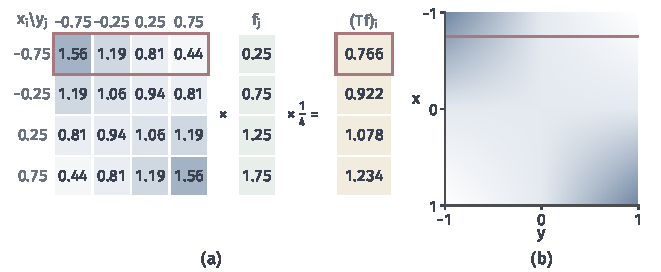
\includegraphics[width=112mm]{figures/04-spaces-measures-and-geometry/03-function-spaces/matplotlib/lop-kernel-as-matrix/figure.pdf}
  \caption{积分算子是矩阵的连续版本，核$k(x,y)=1+xy$就是矩阵元素。(a)四个中点上的矩阵$K_{ij}=1+x_ix_j$，乘以输入$f=1+x$的取值（绿）和格子测度$1/4$，得到输出的近似值（黄）；红框是第一行与它给出的输出。(b)同一个核在连续变量下的取值，纵轴向下对应行号，颜色越深值越大，红线是$x=-3/4$的一行。}
  \label{fig:lop-kernel-as-matrix}
\end{BookInlineFigure}

图中(b)是把格子无限加细后的样子。行变成水平切片，矩阵元素变成曲面上的一点，$k(x,\cdot)$作用于输入的方式与(a)中的第一行相同。

这个对应在哪里失效，也应当说清楚。恒等算子的矩阵是对角线上全为$1$。对角线$\{x=y\}$在正方形中面积为零，任何函数形式的核都承载不了它，所以恒等算子在$L^2(0,1)$上不是积分算子。求导相当于差分矩阵，同样只有对角线附近的元素，也没有函数形式的核。

\paragraph{微分}
在$[0,1]$上令$Df=f^\prime$。连续函数未必可导，例如$f(x)=\lvert x-1/2\rvert$在$x=1/2$处没有导数，所以$D$不能定义在整个$C[0,1]$上。

取定义域$D(D)=C^1[0,1]$，即导数存在且连续的函数，输出$f^\prime\in C[0,1]$，线性来自求导的线性。于是求导是一个从$C[0,1]$到$C[0,1]$、定义在真子空间$C^1[0,1]$上的线性算子。它也可以看成从$C^1[0,1]$到$C[0,1]$的算子，两种看法的区别要到配置范数时才显现出来。

这些例子中，恒等、投影与乘以有界函数自然定义在整个空间上；积分变换须由核与测度的条件保证定义；求导只能定义在一部分函数上。下一节为输入与输出配上范数，研究这些算子是否用一个统一的常数控制误差。
